\chapter{디지털 비디오 인터페이스}
\begin{figure*}
    \centering
    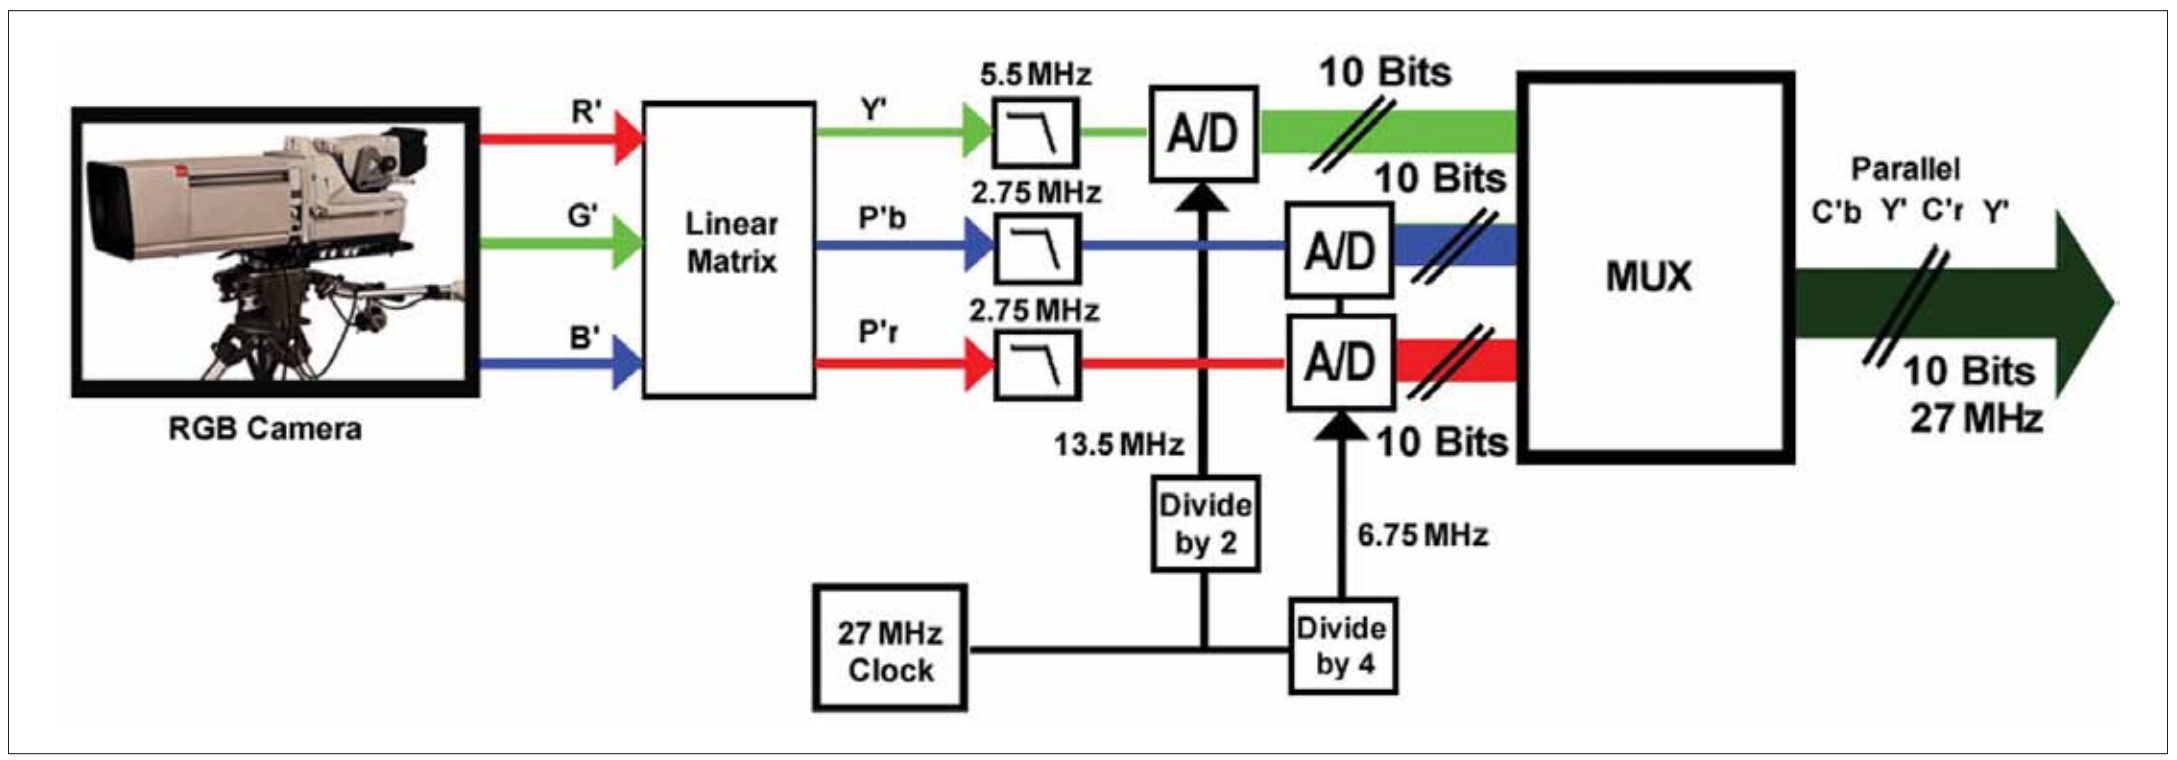
\includegraphics[width=\textwidth]{digitizing rgb camera.PNG}
    \caption{RGB 카메라 신호의 디지털화}\label{fig:digitizing rgb camera}
\end{figure*}
이 시점에서 아날로그 비디오와 연결하는 디지털 인터페이스를 간단히 살펴보는 게 적절하다.
\figurename~\ref{fig:digitizing rgb camera}부터 \figurename~\ref{fig:recovering analog values from prallel data}까지의 블록 다이어그램은 비디오 프로덕션 장비가 디지털 비디오 요소들을 어떻게 다루는지 이해하는 데 도움을 줄 것이다.
이 그림들이 SD 시스템을 다루긴 하지만, 기본 개념은 HD 포맷에서도 똑같다. HD 포맷에서는 샘플링과 데이터 속도가 더 빠르고 각각 분리된 10비트의 휘도와 색차 버스가 시스템 전체에서 더 유지되고, 이를 통해서 고속으로 작동해야 하는 회로를 줄인다.
\\
감마 보정된 RGB(\figurename~\ref{fig:digitizing rgb camera})는 선형 행렬을 통해서 휘도 요소인 Y'과 두 개의 배율이 곱해진 색차 요소인 P'b와 P'r로 바뀐다.
눈은 색상 변화보다 밝기 세부 정보의 변화에 더 민감하므로, Y'신호는 시스템 내에서 더 높은 대역폭으로 전달된다(SD의 경우 5.5 MHz).
휘도와 색차 신호는 샘플링(디지털화) 과정에서 에일리어싱을 일으킬 수 있는 고주파 비디오 성분을 제거하기 위해서 저역 통과 필터로 처리된다.
필터링된 휘도 신호는 아날로그-디지털 변환기에서 13.5 MHz의 속도로 샘플링되어 13.5 Mb/s의 10비트 데이터 스트림으로 바뀐다.
두 개의 색차 신채널들은 필터링된 후 아날로그-디지털 변환기에서 6.75 MHz의의 속도로 2개의 6.75 Mb/s의 데이터 스트림으로 바뀐다.
세 비디오 채널들은 27 Jb/s의 단일 10비트 병렬 데이터 스트림으로 다중화되어 합쳐진다.
\\
\begin{figure*}
    \centering
    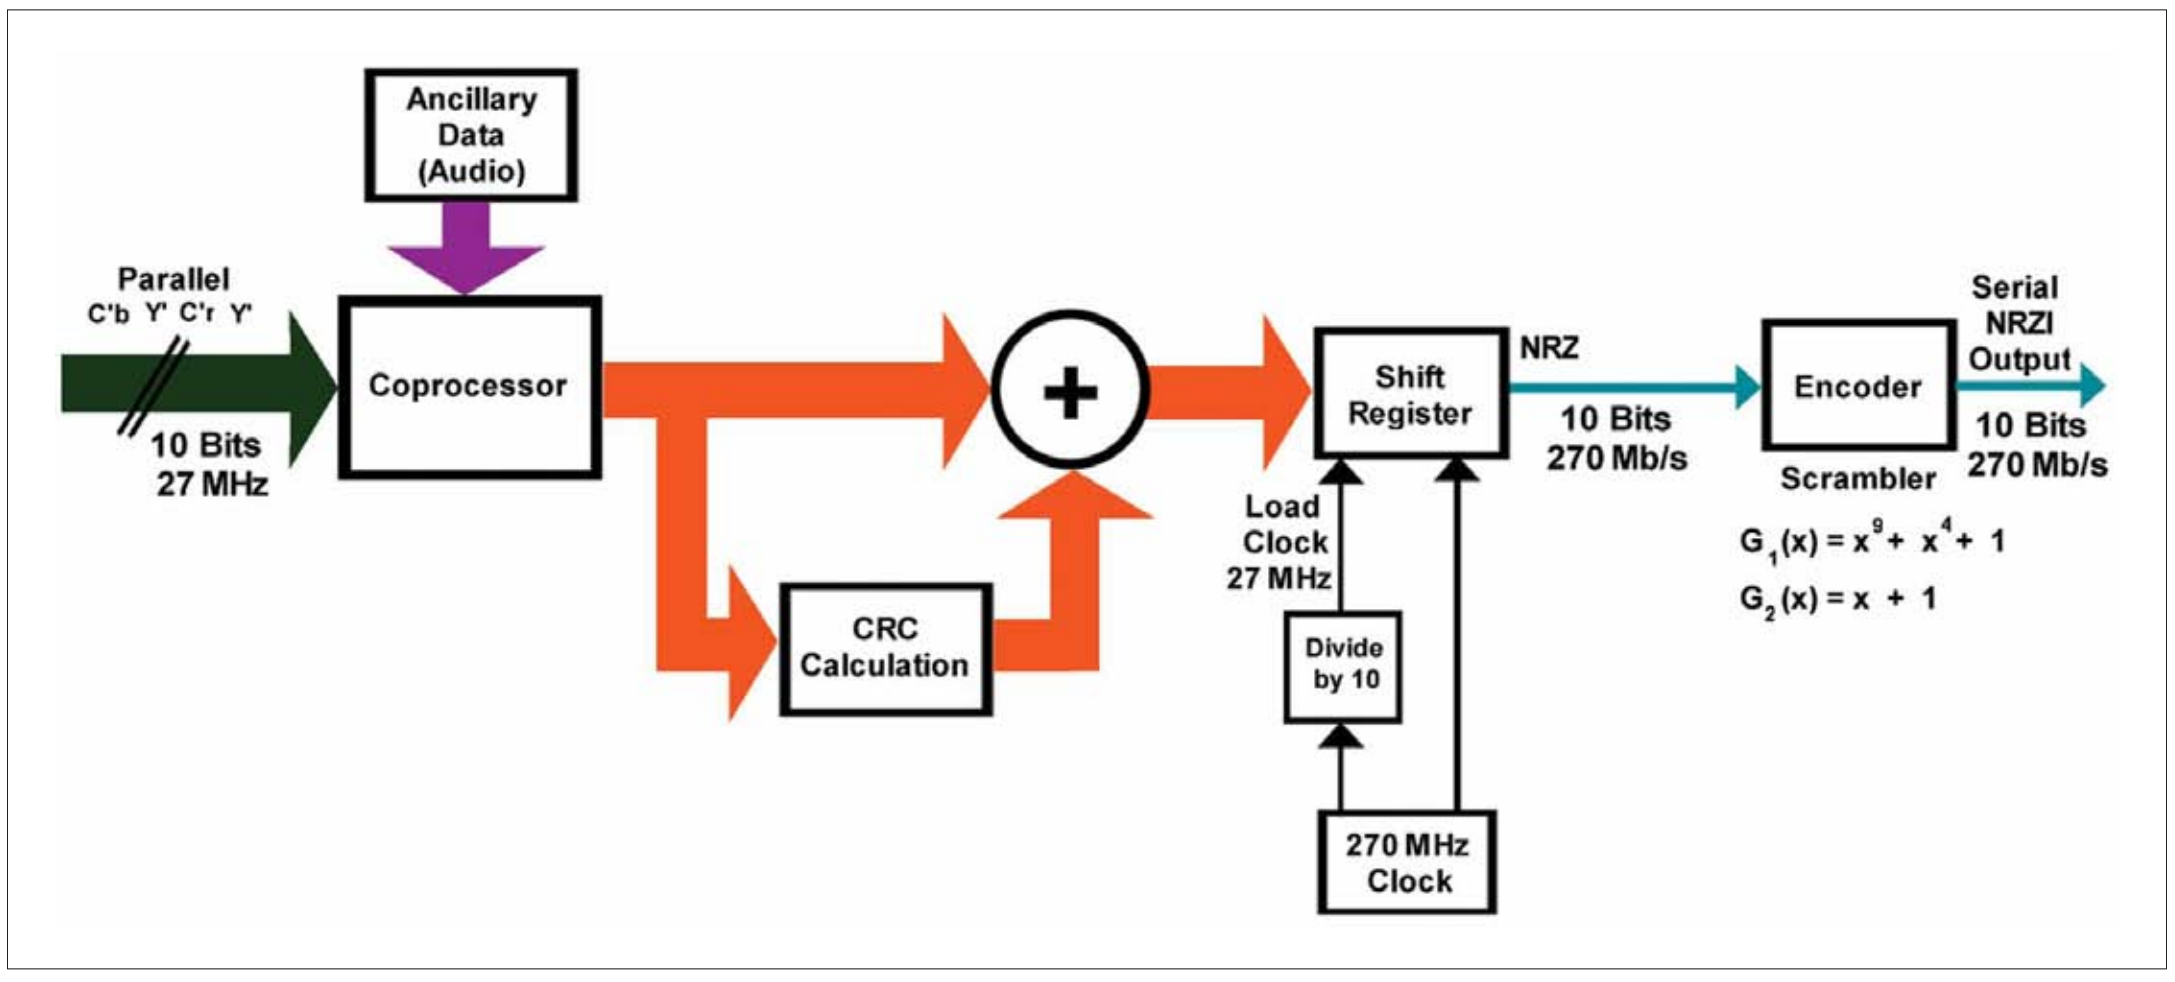
\includegraphics[width=\textwidth]{processing and serializing parallel data stream.PNG}
    \caption{병렬 데이터 스트림의 처리와 직렬화}\label{fig:processing and serializing parallel data stream}
\end{figure*}
보조 처리기(\figurename~\ref{fig:processing and serializing parallel data stream})가 타이밍 기준 신호, AES/EBU 포맷의 디지털 오디오와 기타 부가 데이터를 추가한다. 데이터에 대한 체크섬 또한 계산되어서 병렬 데이터 스트림에 추가된다.
\\
27 Mb/s, 10 비트의 병렬 데이터는 270 Mb/s로 작동하는 시프트 레지스터(또는 직렬화기)로 입력되어서, 이 예제에서는 SD 표준인 ITU-R BT-656/SMPTE 259M을 따르는 적절한 전송을 위해서 스크램블된다.
\\
SD ITU-R BT-656/SMPTE 259M 적합 신호는 표준 비디오 케이블을 따라서 거의 100\%의 무결성을 유지하며 300 m를 갈 수 있다. 1.485 Gb/s의 HD SMPTE 292M 적합 신호는 약 100 m를 갈 수 있다.
\\
\begin{figure*}[!t]
    \centering
    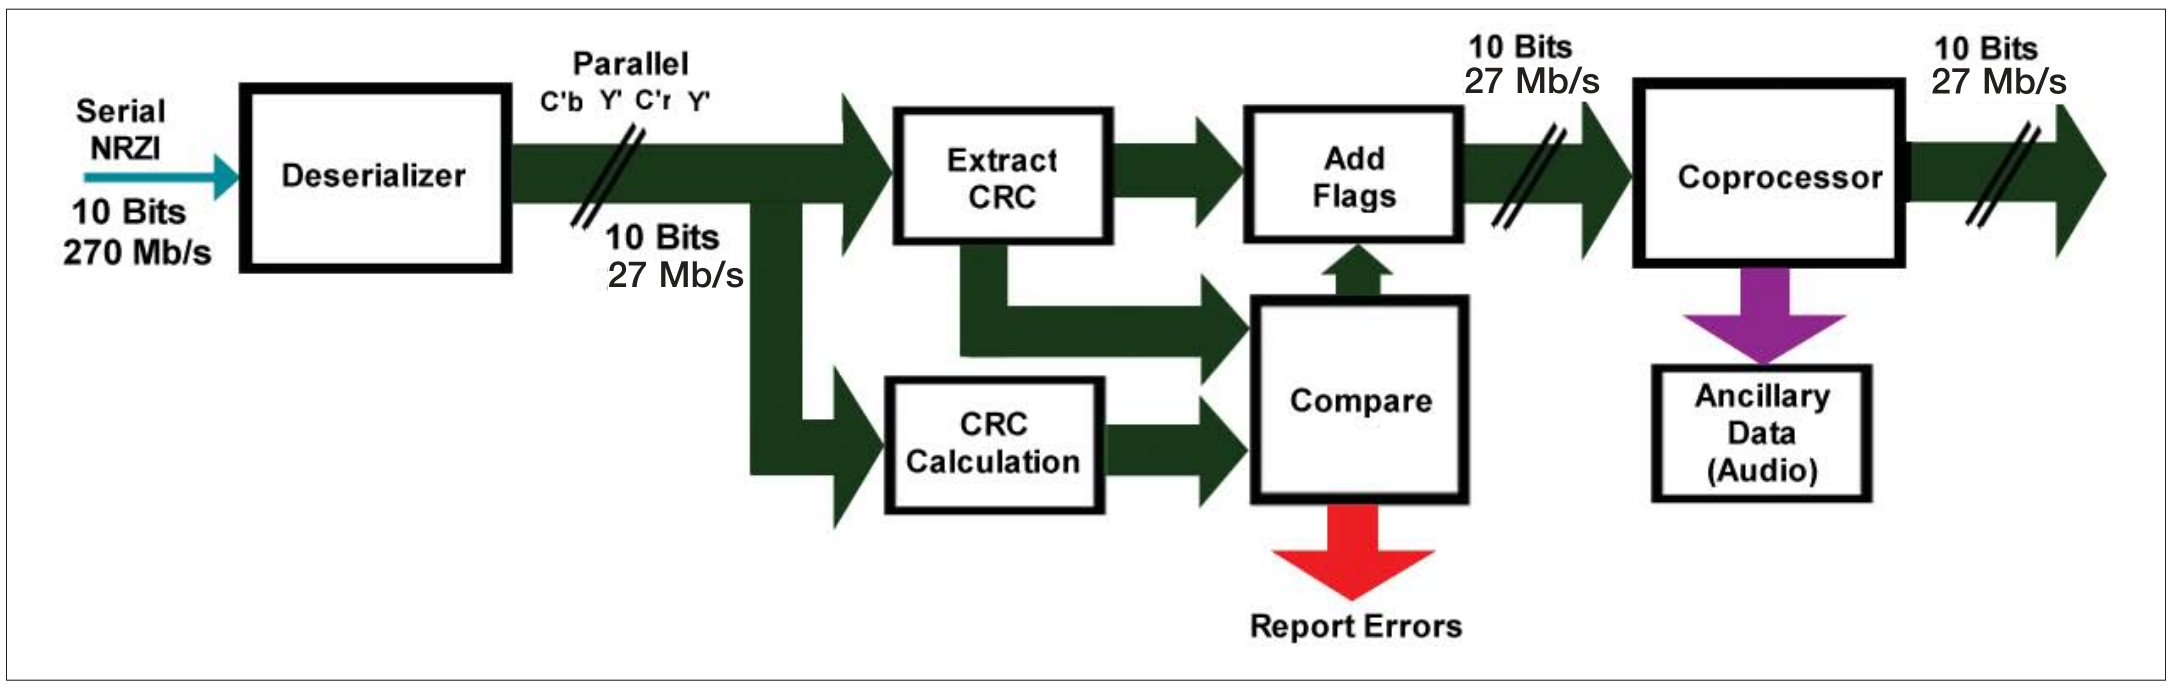
\includegraphics[width=\textwidth]{sdi receiver.PNG}
    \caption{SDI 수신기 - 비디오 데이터를 역직렬화하여 다시 병렬로 만든다}\label{fig:sdi receiver}
\end{figure*}
\begin{figure*}[h!]
    \centering
    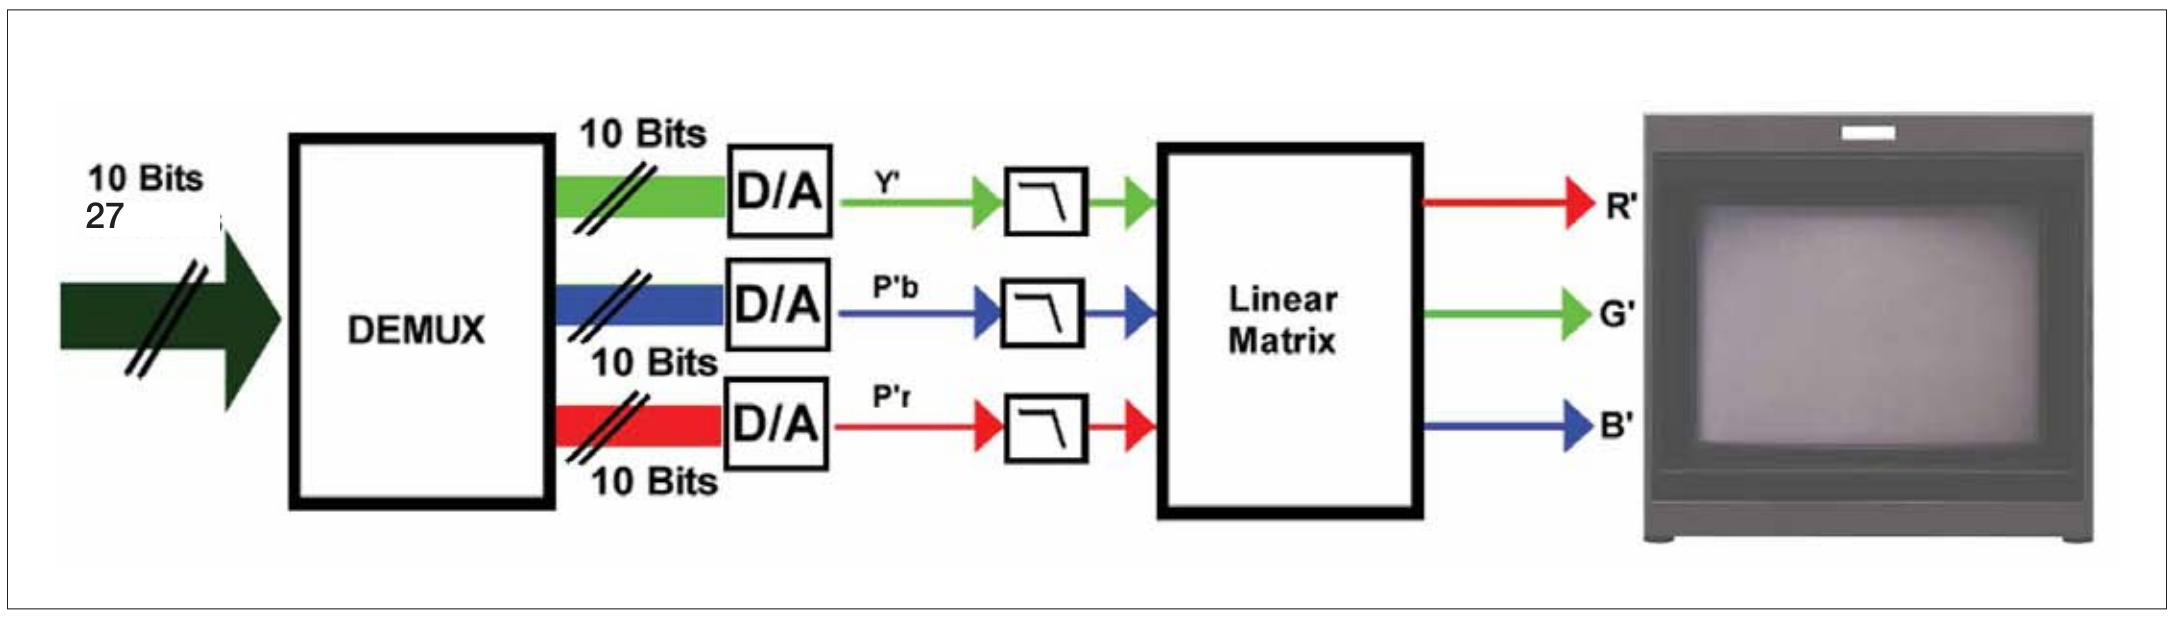
\includegraphics[width=\textwidth]{recovering r'g'b' from parallel data.PNG}
    \caption{병렬 데이터에서 아날로그 R'G'B'를 복원}\label{fig:recovering analog values from prallel data}
\end{figure*}
수상기에서는(\figurename~\ref{fig:sdi receiver}) 절반 클럭 주파수의 에너지가 감지되어서 270 Mb/s로 입력되는 신호를 적절히 아날로그 등화 처리한다. 새로운 270 MHz 클럭이 NRZI(Non-Return to Zero Inverse) 신호의 에지에서 복원되고, 등화된 신호가 논리 상태를 결정하기 위해서 샘플된다.
역직렬화기는 인코더의 스크램블 알고리즘의 역변환을 이용해서 스크램블을 해제하여 27 Mb/s의 10비트 데이터 스트림을 만든다. 임베디드된 체크섬이 수신기에서 추출되어서 수신된 데이터로부터 새로 계산된 체크섬과 비교되어 오류가 발생했는지 확인하고 적절한 플래그를 데이터 스트림에 붙인다.
보조 처리기는 오디오나 다른 부가 데이터들을 추출한다.
\\
10비트 데이터 스트림은 역다중화되어(\figurename~\ref{fig:recovering analog values from prallel data}) 디지털 휘도와 색차 스트림이 되고, 3개의 디지털-아날로그 변환기를 통하여 아날로그 신호가 되며, 이산적인 데이터 레벨에서 부드러운 아날로그 신호가 되도록 (역자 주:저역) 필터를 통과하고 디스플레이에서 원래의 R'G'B'신호가 되게 행렬을 이용해서 합쳐진다.
\\
이 간단한 시스템 개관은 시스템이 어떻게 작동하는지 이해하는 데 도움이 될 것이다. 추가적인 디지털 인터페이스에 대한 세부적인 설명은 뒤의 문단들에서 나올 것이다.

\section{601 샘플링}
\begin{figure*}[t!]
    \centering
    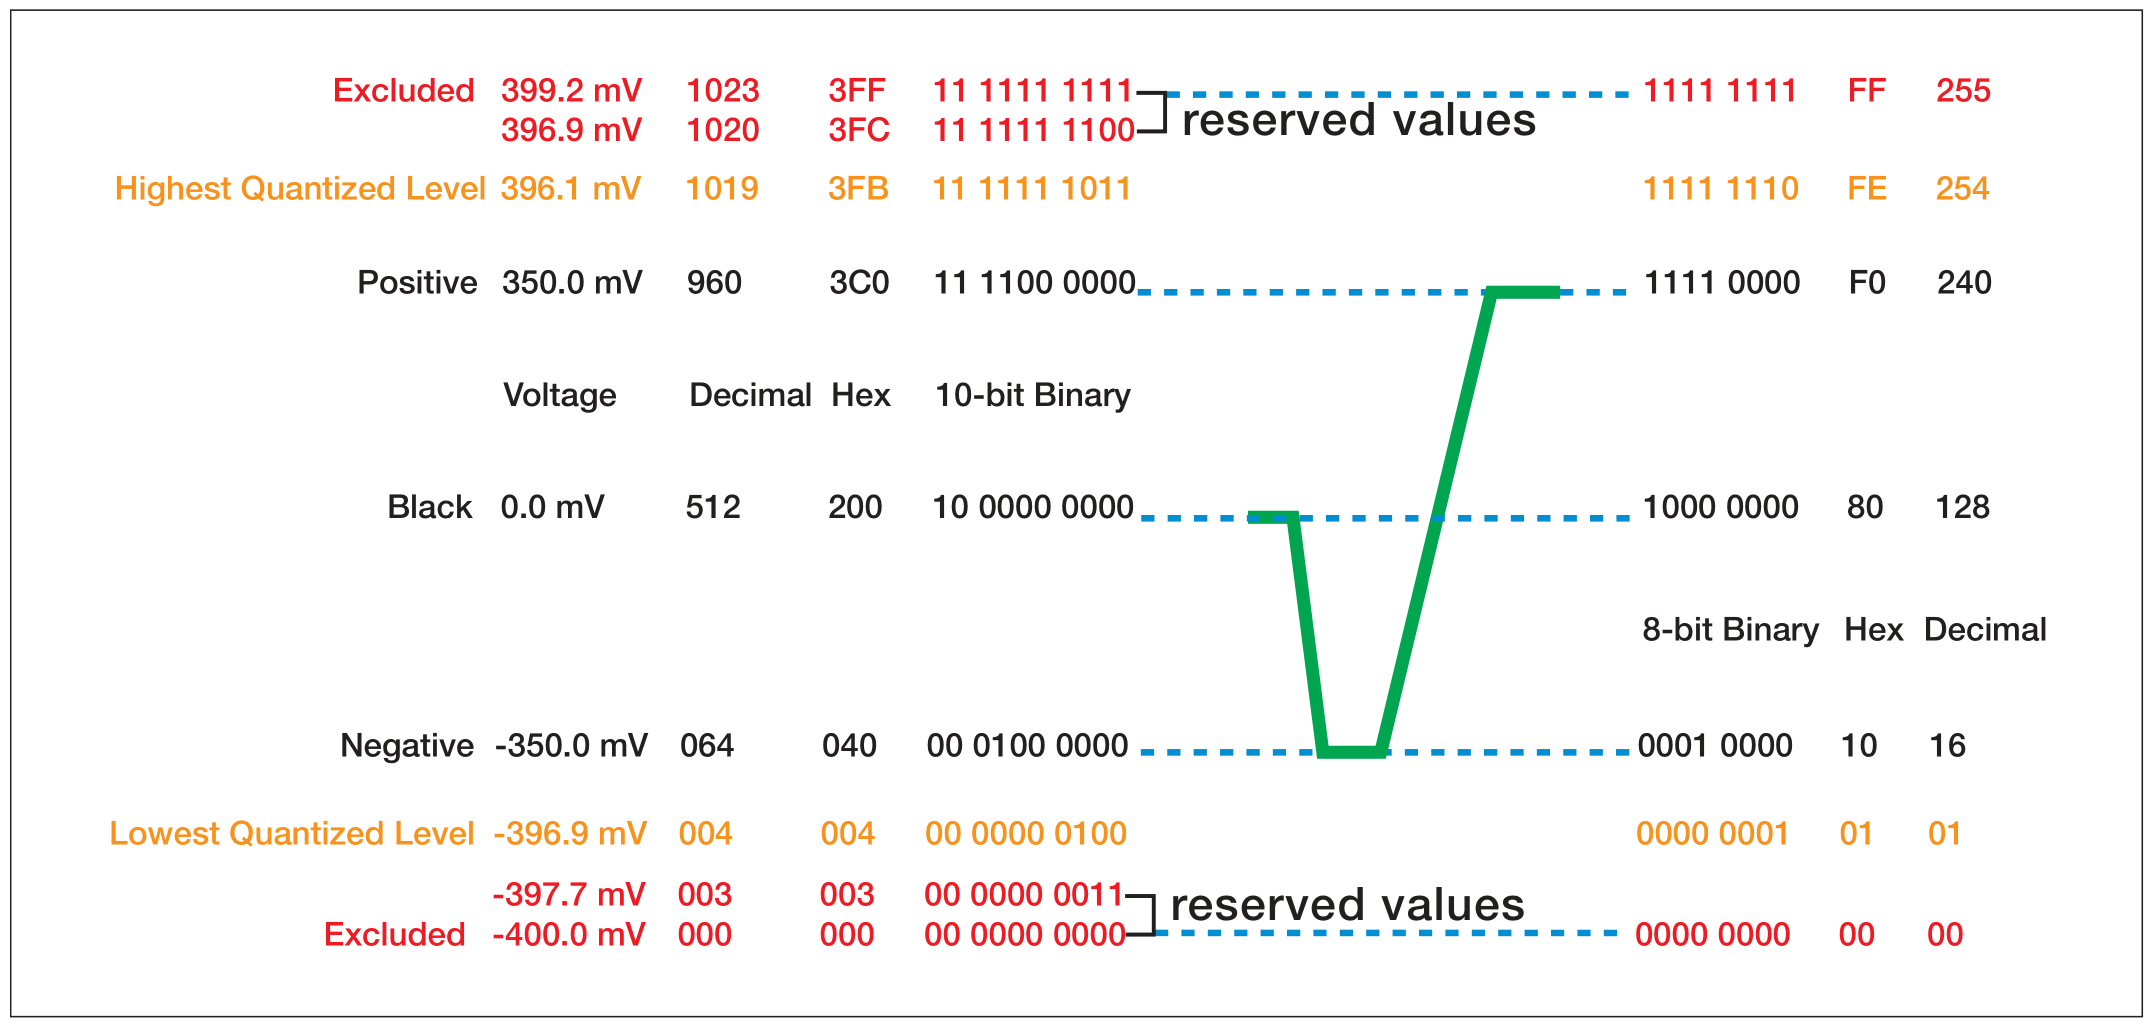
\includegraphics[width=\textwidth]{color difference quantizing.PNG}
    \caption{색차 신호의 양자화}\label{fig:color difference quantizing}
\end{figure*}
\begin{figure*}[h!]
    \centering
    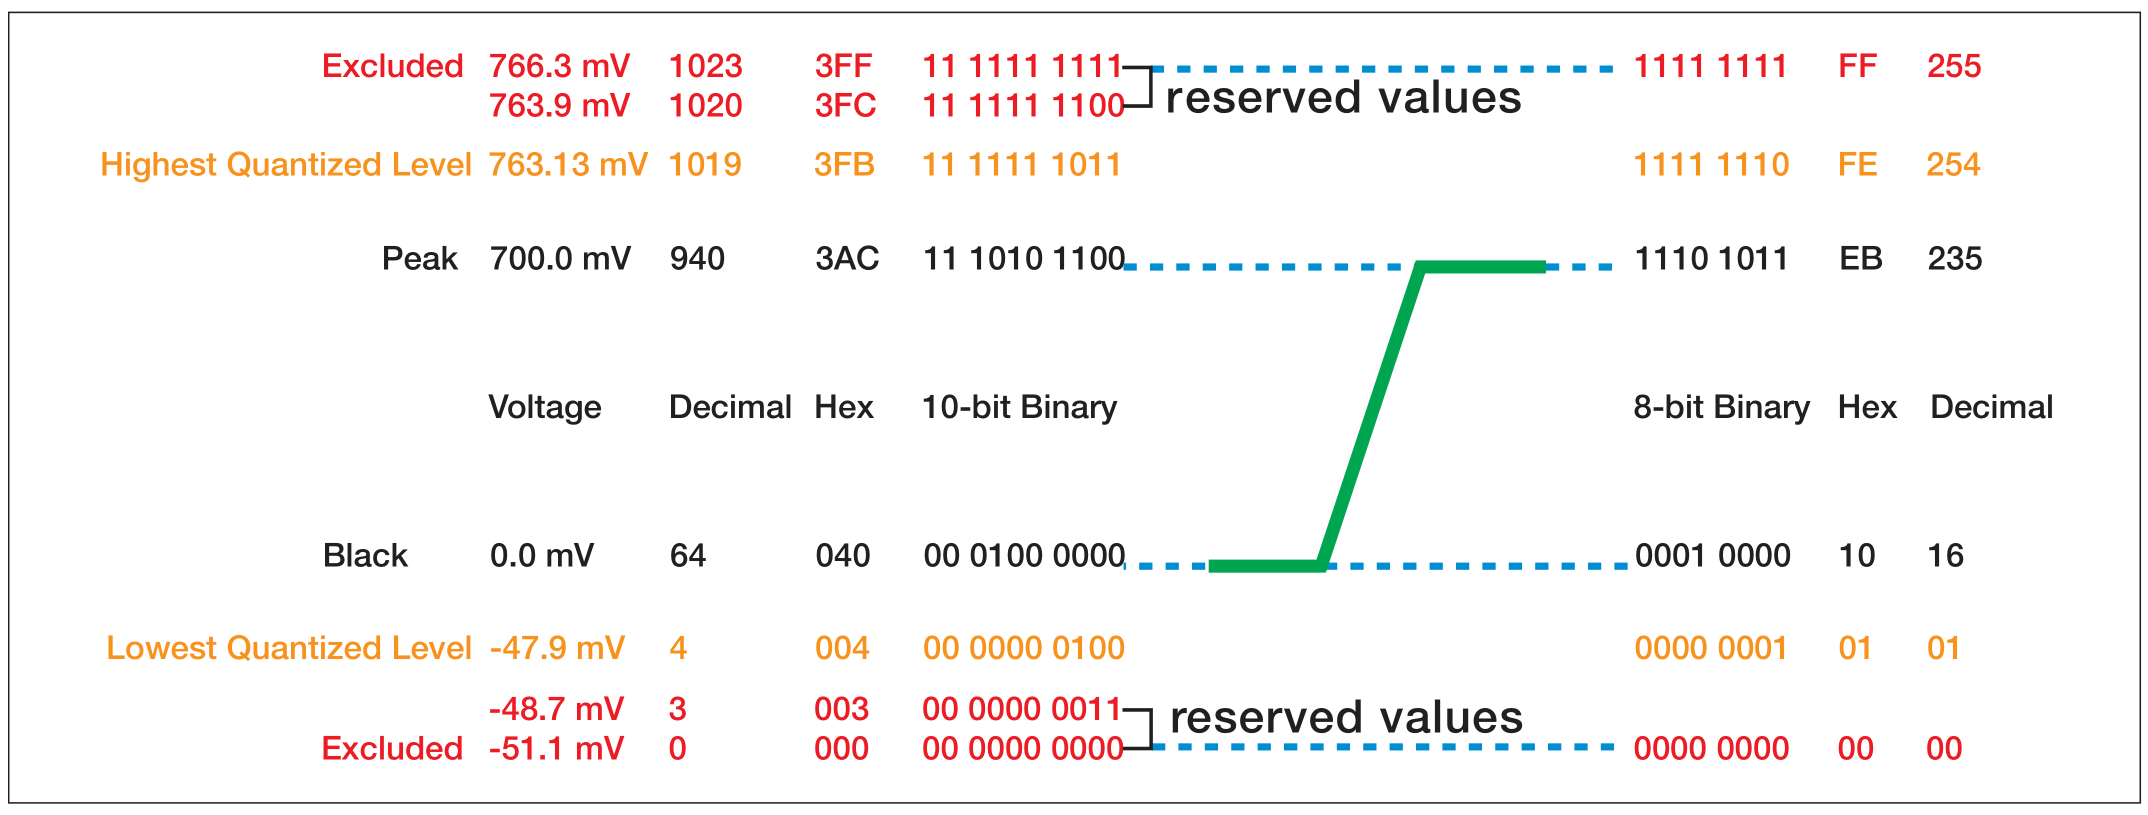
\includegraphics[width=\textwidth]{luminance quantizing.PNG}
    \caption{휘도 신호의 양자화}\label{fig:luminance quantizing}
\end{figure*}
ITU-R BT.601은 625/50과 525/60 텔레비전 시스템의 디지털 요소들에 대한 파라미터를 결정하기 위한 연합 SMPTE/EBU 태스크 포스에서 만들어진 샘플링 표준이다.
이 작업은 1981년에 SMPTE에 의해 후원된 일련의 테스트들로 완결되었고, 잘 알려진 CCIR 권고안 601 (이제는 ITU-R BT.601)이라는 결과가 나왔다.
이 표준 문서는 525와 625줄 신호에서 사용되는 샘플링 방법을 규정한다. 이는 아날로그 휘도에 대한 13.5 MHz와 두 개의 아날로그 색상차 신호에 대한 6.75 MHz의 직교 샘플링을 규정하고 있다.
샘플링된 값들은 디지털 휘도인 Y'와 디지털 색차 신호인 C'B와 C'r인데 이들은 아날로그의 감마 보정 신호인 B'-Y'와 R'-Y'에 배율이 곱해진 것이다.
525줄과 625줄 시스템에서 공통적인 요소인 2.25 MHz가 13.5 MHz의 약수이기 때문에 13.5 MHz라는 샘플링 주파수가 선정되었다(부록 B - 텔레비전 클럭 관계를 참고하라).
\\
현재 많은 ITU-R BT.601 구현들이 10 비트 샘플링을 쓰고 있지만, ITU-R BT.601은 8비트 샘플링($00_h$부터 $FF_h$까지 256레벨을 갖는)과 10비트 샘플링($000_h$부터 $3FF_h$까지 1024 레벨을 갖는) 모두를 허용한다.
8비트 워드는 바로 10비트로 변환될 수 있고, 10비트 값은 8비트 시스템과의 상호 운용성을 위해 8비트로 반올림된다. 색차 성분 C'r과 C'b 값들은 $\pm 350$ mV에 대응되는 $040_h$부터 $3C0_h$까지의 값을 갖는다.
이 범위를 넘어서는 신호도 허용되고, 최종적으로 가능한 범위는 $\pm 400$ mV이다. 휘도 성분 Y' (\figurename~\ref{fig:luminance quantizing})의 값의 범위는 $040_h$부터 $3AC_h$의 값을 갖는데 이는 아날로그 신호의 0.0 mV부터 700 mV까지에 대응된다.
이 범위를 벗어나는 신호도 마찬가지로 허용되고, 흰색 레벨을 넘어서는 과한 값을 처리할 수 있는 더 넓은 여유 공간을 위해 최종적인 범위는 -48 mV부터 +763 mV까지가 된다.
아날로그/디지털 변환기들은 $000_h$부터 $003_h$와 $3FC_h$부터 $3FF_h$의 10비트 값을 생성하지 않도록 설정되는데 이는 8비트 시스템과의 상호 운용성을 위해서이다.
양자화 레벨은 8비트 레벨에 두 개의 0을 붙이면 10비트 값과 같은 값이 되도록 선택된다. 휘도와 색차 아날로그/디지털 컨버터 모두에서 $000_h$부터 $003_h$와 $3FC_h$부터 $3FF_h$까지의 값은 동기화를 위해 예약되어 있다.
\\
\begin{figure}[!htp]
    \centering
    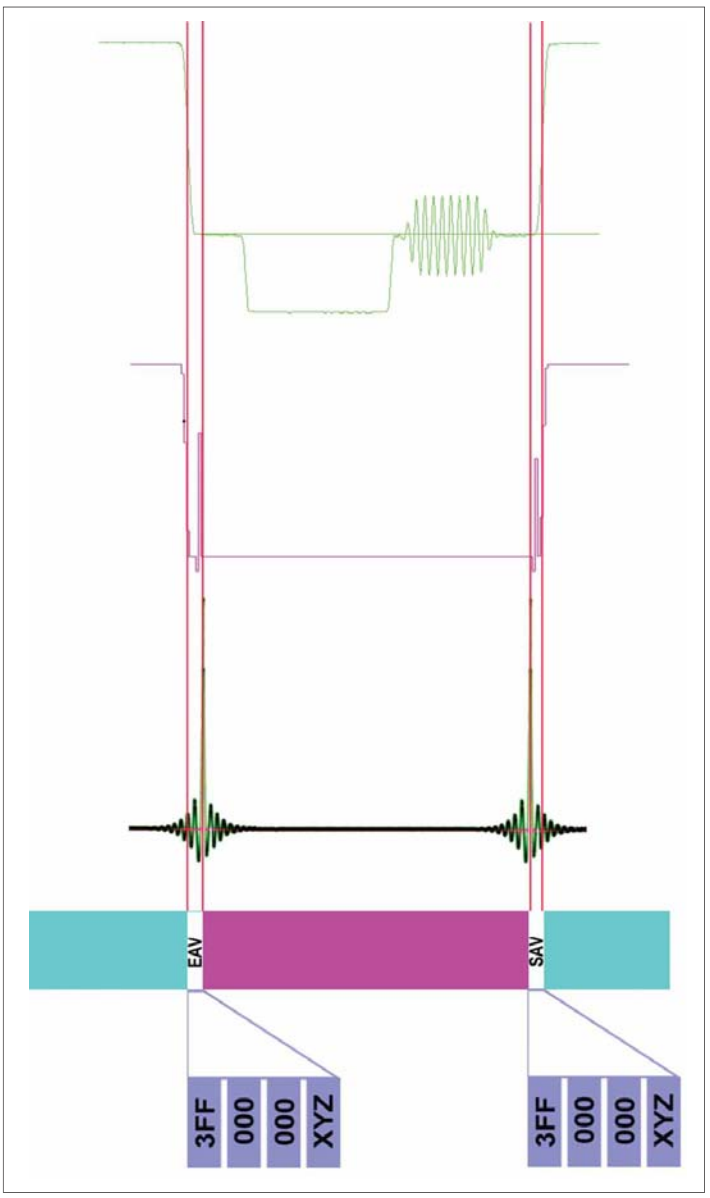
\includegraphics[width=0.4\textwidth]{digital horizontal blanking interval.PNG}
    \caption{디지털 수평 블랭킹 구간}\label{fig:digital horizontal blanking interval}
\end{figure}
\begin{figure*}[tpb]
    \centering
    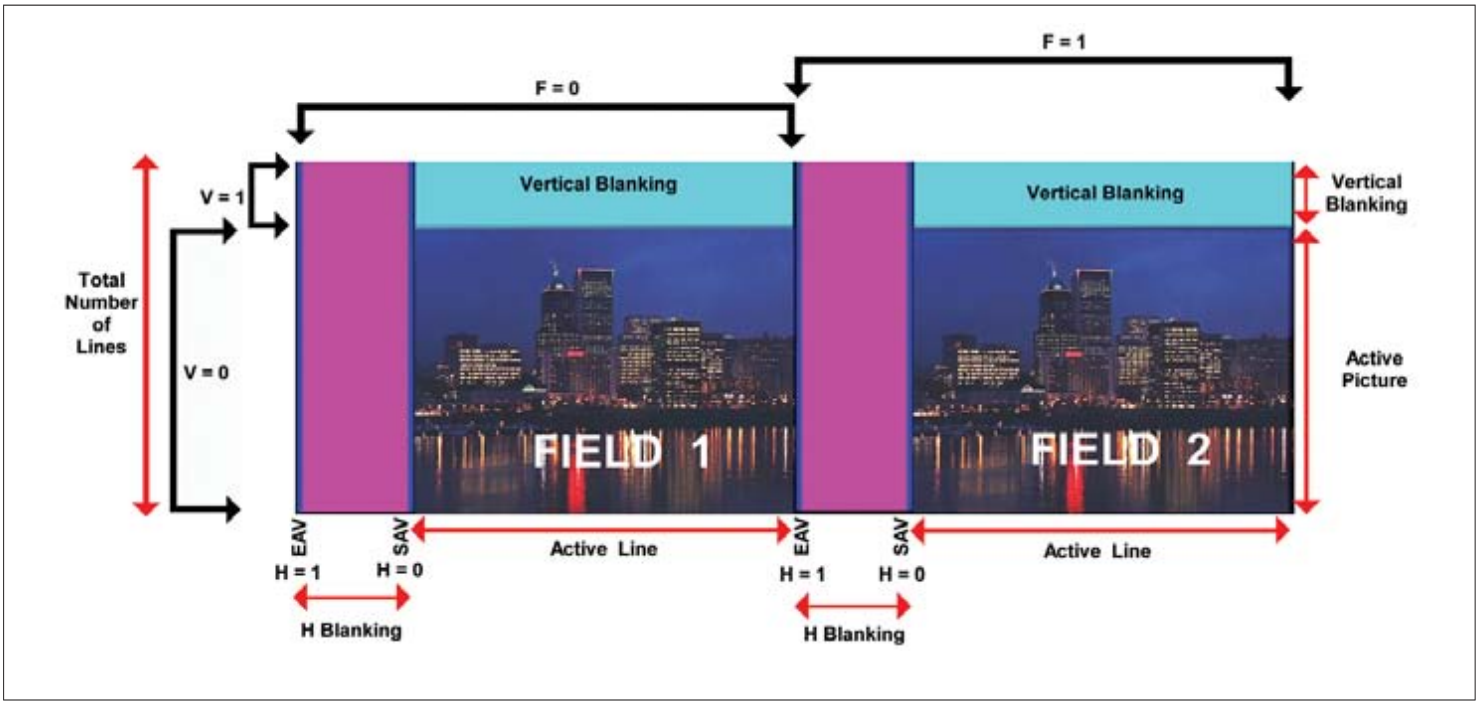
\includegraphics[width=\textwidth]{layout of 2 to 1 interlaced digital frame.PNG}
    \caption{2:1 비월 주사 디지털 프레임의 구조}\label{fig:layout of 2:1 interlaced digital frame}
\end{figure*}
\figurename~\ref{fig:digital horizontal blanking interval}\은 아날로그 수평 선에 대응되는 샘플들과 디지털 워드들의 위치를 보여주고 \figurename~\ref{fig:layout of 2:1 interlaced digital frame}\은 그림 영역과의 공간적인 관계를 보여준다.
타이밍 정보는 활성 비디오의 끝(EAV;End of Active Video)와 활성 비디오의 시작(SAV;Start of Active Video) 패킷이 전달하기 때문에 전통적인 동기화 신호는 필요하지 않다.
수평 블랭킹 구간과, 수직 블랭킹 구간의 전체 선 구간동은 오디오나 기타 부가 데이터를 전달하는 데 쓰일 수 있다. EAV와 SAV 타이밍 패킷은 데이터 스트림에서 $3FF_h, 000_h, 000_h$라는 워드로 시작하는 헤더로부터 알아낼 수 있다.
\\
"xyz"워드는 8비트 신호 경로에서 문제 없이 전달될 수 있게 2개의 가장 중요하지 않은 비트(역주: 끝의 2비트)가 0으로 설정된 10비트 워드이다.
SD에서 "xyz"워드들은 F ,V ,H라는 함수를 담고 있는데, 각 함수들은 다음의 값을 갖는다:
\begin{itemize}
    \item 8번째 비트 - (F비트) 첫 번째 필드에서 0, 두 번쨰 필드에서 1
    \item 7번째 비트 - (V비트) 수직 블랭킹 구간에서 1, 활성 비디오 선에서 0
    \item 6번째 비트 - (H비트) 1은 EAV 시퀀스를 가리키며 0은 SAV 시퀀스를 가리킴
\end{itemize}

\section{병렬 디지털 인터페이스}
Rec.601 샘플링에 의해 생성된 데이터의 전기적 인터페이스는 525/59.94를 위한 SMPTE 125M 표준과 625/50을 위한 EBU Tech. 3267로 별도로 표준화되었다. 두 표준 모두 CCIR(현 ITU)가 채택했고 병렬 하드웨어 인터페이스를 설명하는 권고안 656에 포함되었다.
병렬 인터페이스는 11개의 꼬인 쌍과 25개의 D 커넥터를 이용한다. 병렬 인터페이스는 데이터 워드들을 다중화하여 27 Mb/s의 속도의 C'b, Y', C'r, Y, ...의 시퀀스로 만든다. 타이밍 시퀀스인 SAV와 EAV가 각 선에 추가된다.
525와 625 포맷 모두의 디지털 활성 비디오 선은 720개의 휘도 샘플을 포함하는데, 남는 샘플들은 아날로그 블랭킹에 해당하며 타이밍과 기타 데이터에 이용될 수 있다.
\\
여러 전선과 패치 패널을 이용해야 하기 때문에, 디지털 스튜디오 장비들을 병렬로 연결하는 것은 작고 영구적으로 구성된 시스템에서만 현실적으로 이용할 수 있다.

\section{직렬 디지털 인터페이스(SDI)}
\begin{figure}
    \centering
    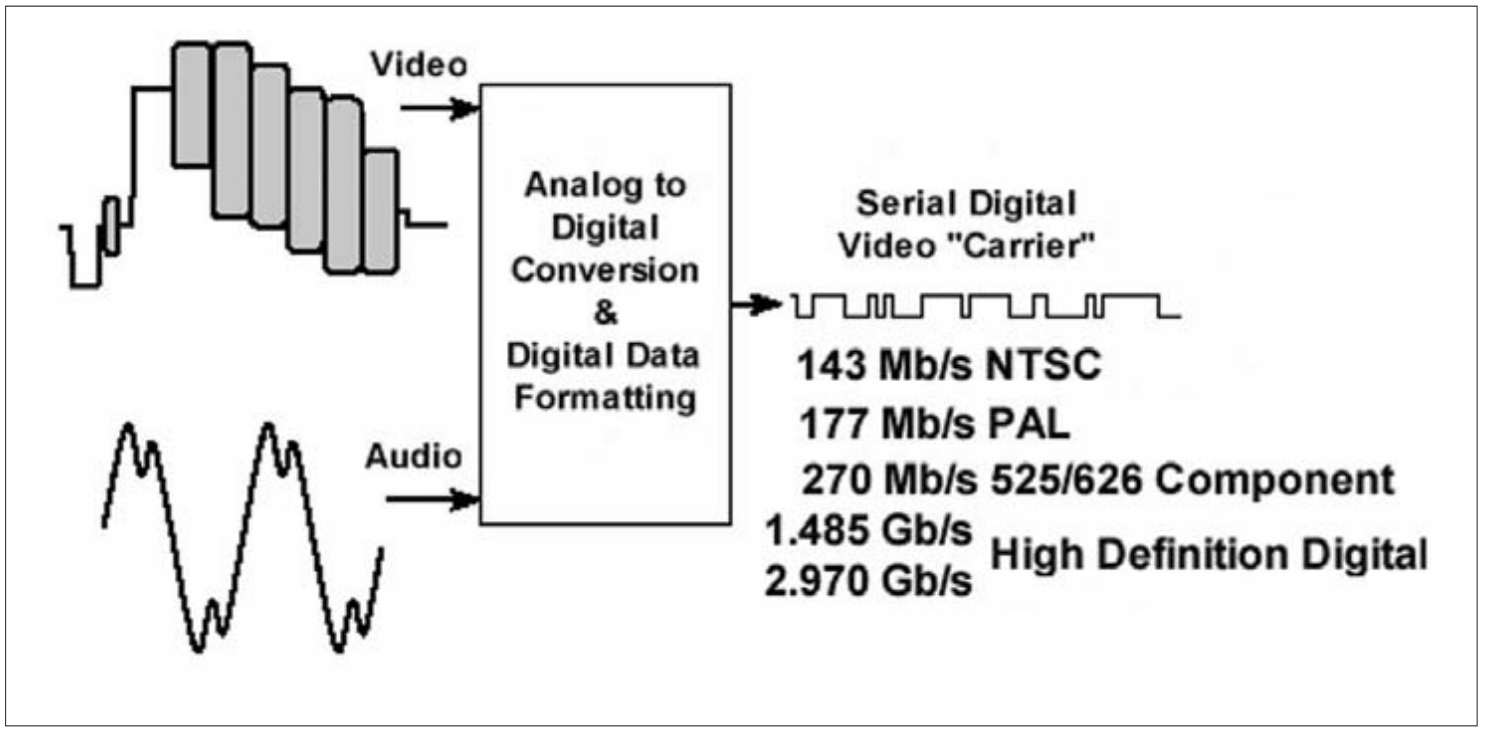
\includegraphics[width=0.5\textwidth]{the carrier concept.PNG}
    \caption{반송파 개념}\label{fig:the carrier concept}
\end{figure}
포맷과 상관없이 하나의 동축 케이블만으로 데이터를 보낼 필요가 분명히 있다. 이는 데이터 속도가 비교작 높아서뿐만이 아니라 신호가 적절히 변형되지 않으면 신뢰성 있는 복구가 어렵기 떄문이다(역주: 동기화가 필요하다).
신호는 전송 전에 신뢰성 있는 클럭 복구가 가능하게 충분히 많은 에지를 포함하고, 전송된 신호에 저주파 성분이 최소화되게 하고(역주: 시스템의 각 단은 보통 커패시터로 커플링되므로), 에너지 스펙트럼이 골고루 퍼져서 RF 방출 문제가 최소화되도록 변형되어야 한다.
스크램블링과 NRZI로의 변환을 이용하는 직렬 디지털 인터페이스가 이러한 요구사항을 만족시키기 위해 개발되었다. 이 시리얼 인터페이스는 ANSI/SMPTE 259M, ITU-R BT.656과 EBU Tech. 3267에 규정되어 있는데, SD 컴포넌트와 임베디드된 디지털 오디오를 포함하는 컴포지트 신호 모두에 대한 것이다.
이 직렬 인터페이스의 확대된 버전이 HD 전송을 위해서 규정되어 있다.
\\
개념적으로, 직렬 디지털 인터페이스는 스튜디오에서 응용되는 반송파 시스템과 유사하다. 기저대역 비디오와 오디오 신호는 디지털화되고 \figurename~\ref{fig:the carrier concept}에서 보여지는 것처럼 직렬 디지털 반송파 위에서 합쳐진다.
이 신호는 기저대역 디지털 신호이지 반송파 위에 변조된 게 아니라는 점에서 엄격히는 반송파 시스템이 아님을 명심하라.
비트율(반송파 주파수)는 디지털 데이터의 클럭으로 정해지는데, SD 컴포넌트 디지털에 대해서는 270 Mb/s이고 HD에 대해서는 1.485 Gb/s(또는 2.97 Gb/s)이다. (NTSC와 PAL 컴포지트 직렬 인터페이스의 143 Mb/s와 177 Mb/s 등 다른 속도도 사용되지만 여기서 자세히 다루지는 않겠다.)\
\\
\begin{figure}
    \centering
    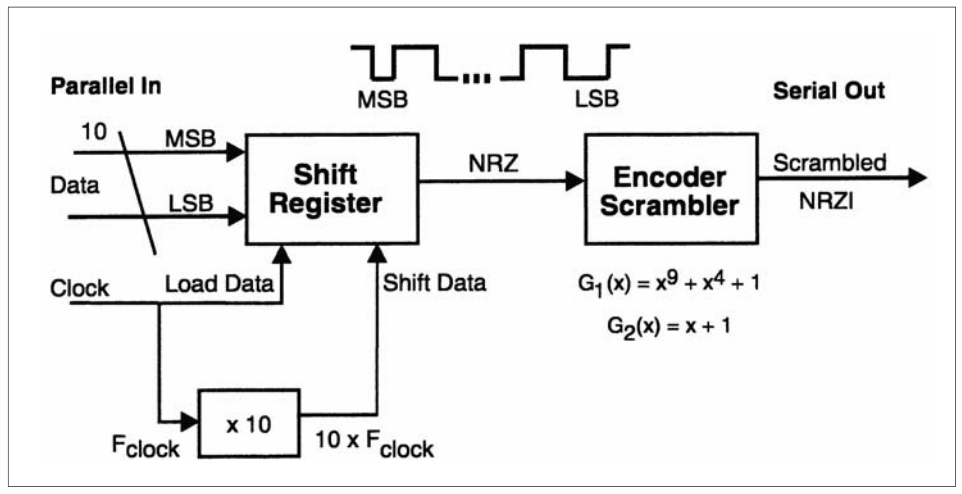
\includegraphics[width=0.5\textwidth]{parallel to serial conversion.PNG}
    \caption{병렬에서 직렬로 변환}\label{fig:parallel to serial conv}
\end{figure}
\begin{figure}
    \centering
    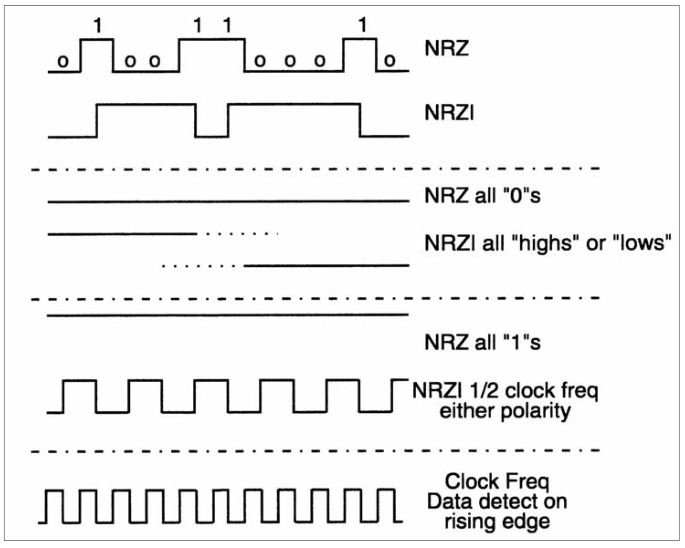
\includegraphics[width=0.5\textwidth]{nrz and nrzi.PNG}
    \caption{NRZ와 NRZI의 관계}\label{fig:nrz and nrzi}
\end{figure}
아날로그 신호 성분들을 표현하는 병렬 데이터는 \figurename~\ref{fig:parallel to serial conv}\와 같이 처리되어 디지털 데이터 스트림이 된다. 병렬용 클럭이 샘플 데이터들이 시프트 레지스터로 입력되는 데에 사용되고, 병렬용 클럭의 10배의 클럭이 각 10비트 워드들에 대해 LSB를 가장 먼저로 하여 비트들을 출력한다.
8비트 데이터만 가능하다면 직렬화기는 두 개의 LSB에 0을 채워서 10비트 워드를 완성한다. 컴포넌트 포맷에서는 병렬 인터페이스의 EAV와 SAV 타이밍 신호가 유일한 시퀀스를 만들어서 직렬 영역에서 이들을 이용해서 워드들을 프레임 단위로 만들 수 있게 한다.
EAV와 SAV 데이터 패킷을 코딩하는 방법은 이 글의 디지털 스튜디오 동기화 및 타이밍 장에 설명되어 있다. 오디오와 같은 다른 부가 데이터가 병렬 신호에 삽입되어 있다면, 이 데이터 또한 직렬 인터페이스에 의해 전달될 것이다.
\\
병렬 정보의 직렬화 뒤에는 데이터 스트림이 수학적 알고리즘에 의해 스크램블되고, 그 후에는 다음의 두 함수의 합성에 의해 NRZI로 인코딩된다.
\begin{IEEEeqnarray*}{lCr}
    G_1(X)=X^9+X^4+1$$\\
    G_2(X)=X+1$$
\end{IEEEeqnarray*}
스크램블링을 하면 통계적으로 신호가 적은 직류 성분을 갖게 되고 이는 신호를 다루기 쉽게 만든다. 또한 많은 상태 전환을 만들어내는데 이로부터 클럭 복구가 용이해진다. NRZI 포매팅은 신호의 극성이 중요하지 않게 만들어준다.
\\
수상기에서 역직렬화기는 이 알고리즘의 역 알고리즘을 이용해서 올바른 데이터를 복원해서 최종 시청자가 원래의 스크램블되지 않은 화면을 보게 해준다. 직렬 디지털 전송 시스템에서는 클럭이 별도 선으로 전달되는 병렬 시스템에서와는 달리 데이터 내에 클럭이 들어있다.
데이터를 스크램블링함으로써, 클럭 복원에 필요한 많은 상태 변환이 보장된다. 시스템의 스트레스 테스트를 위해서(디지털 시스템 테스팅 장을 보라) 높은 직렬 성분과 최소한의 상태 전환으로 이루어진 시퀀스를 갖는 신호가 특별히 고안되어서 SDI 수상기 회로의 성능을 테스트하는 데에 이용된다.
일반적으로 작동하는 직렬 디지털 시스템은 이러한 까다로운 신호에 대해서도 작동할 것이다.
\\
NRZI로 인코딩하는 것은 직렬 데이터가 극성에 민감하지 않도록 해준다. NRZ(Non-Return to Zero)는 친숙한 로직 레벨인 하이="1", 로우="0"을 이용한다. 전송 시스템에서는 수상기가 신호의 특정한 극성에 의존하지 않게 하는 것이 편리하다.
\figurename~\ref{fig:nrz and nrzi}에서 볼 수 있는 것처럼, 데이터 상태 전환이 데이터 "1"을 표현하고, 데이터 "0"에서는 상태 전환이 없다. 그 결과로 신호가 어떤 극성을 띠든 상태 전환만 감지하면 된다. NRZI 인코딩의 또 다른 결과는 모든 "1" 신호는 매 클럭 구간마다 상태 전환을 만들어내고 이는 클럭 주파수의 1/2에 해당하는 사각파를 만들어낸다.
하지만 "0"은 아무 상태 전환을 일으키지 않으므로 스크램블링이 필요하게 된다. 수상기는 클럭 주파수의 사각파의 상승 에지에서 데이터를 감지할 것이다.
\\
직렬 디지털 인터페이스는 75 옴의 비디오 케이블, 커넥터와 패치 패널을 이용하는 잘 설계된 시스템에서는 적당한 거리의 신호 전송에 이용될 수 있다. 예를 들어, T-커넥터에서 볼 수 있는 종단 처리가 되지 않은 케이블의 영향은 아날로그 비디오에서는 보이지 않을지 모르나 직렬 디지털 비디오에서는 미묘한 영향을 끼치고 잠재적으로 프로그램이 제대로 전달되지 않을 수 있다.
\\
병렬과 직렬 컴포넌트 비디오에 대한 논의는 일반적으로 SD와 HD 주사 포맷 모두에 적용될 수 있다. 샘플링과 양자화 레벨은 일반적으로 똑같고, 동기 정보 또한 같다. 샘플링 속도는 더 높아서 일반적으로 HD 포맷에서는 부가 데이터에 대한 더 많은 샘플링이 가능하다.
라인 번호와 오류 확인 워드들이 HD 포맷에 들어있고, 다채널 오디오를 위한 더 많은 샘플들도 들어갈 수 있다. 하지만 기본 원리는 SD와 HD 모두에서 같다. 하나의 컴포넌트 디지털 포맷을 이해하는 것은 다른 것을 전부 이해하는 바탕이 된다.
이 글은 논의를 계속하면서 차이점들을 지적할 것이다. 디지털 SD와 HD 주사 포맷은 타이밍과 동기화 장에서 논의되고 비교될 것이다.

\section{HD 비디오는 SD의 원리에 기반한다}
디지털 HD로 넘어갈 때 우리는 SD에 대해 배운 것을 활용할 수 있고 이를 HDTV의 특정 요구조건에 적용할 수 있다. 아날로그 신호를 샘플링하는 것은 근본적으로 같고, 단지 더 넓은 채널 대역폭과 샘플링 속도를 쓸 뿐이다.
디지털 신호를 처리하는 것도 같고, 차이는 더 높은 데이터 속도를 쓰고 시스템 설계를 더 잘 해야 하는 것 뿐이다. 선을 따라서 모든 게 더 빠른 데이터 속도와 넓은 대역폭으로 작동하지만, 거의 모든 원리들은 비슷하다.
\\
다양한 HD 포맷이 존재한다. 이로써 방송 엔지니어는 방법 선택에 있어 유연성을 갖게 되지만, 시스템 설계는 눈에 띄게 어려워진다.
\\
표준들은 HD 비디오를 만들고 다루는 데 필요한 주사 포맷, 아날로그 인터페이스, 병렬 디지털 인터페이스와 직렬 디지털 인터페이스를 정의한다. 관심을 가져야 하는 중요한 표준들은 다음과 같다.
\begin{itemize}
    \item ANSI/SMPTE 240M. 텔레비전 - 신호 파라미터들 - 1125 주사선 HD 제작 시스템: 60 Hz와 59.94 Hz 필드율의 1125 주사선(활성 1035) 제작 시스템에서 작동하는 최초 영상 생성 장비들의 아날로기 비디오 신호에 대한 기본적인 특성을 정의한다.
    \item SMPTE 260M, 텔레비전 - 디지털 표현과 비트-병렬 인터페이스 - 1125/60 HD 제작 시스템: ANSI/SMPTE 240M에 의해 아날로그 형태로 정의되는 1125/60 HD 신호 파라미터의 디지털 표현을 정의한다.
    \item ANSI/SMPTE 274M, 텔레비전 - 다양한 영상률을 위한 1920 x 1080 주사 및 병렬 디지털 인터페이스: 16:9의 종횡비와 1920 x 1080 크기의 활성 그림 영역을 갖는 주사 시스템들에 대해 정의한다.
    \item ANSI/SMPTE 292M, 텔레비전 - HD 텔레비전 시스템을 위한 비트-직렬 디지털 인터페이스: 1.485 Gb/s와 1.485/1.001 Gb/s로 동작하는 HD 컴포넌트 신호에 대한 비트-직렬 디지털 동축 인터페이스와 광섬유 인터페이스에 대해 정의한다.
    \item ANSI/SMPTE 296M, 텔레비전 - 1280 x 720 주사, 아날로그 및 디지털 표현과 아날로그 인터페이스: 16:9의 종횡비와 1280 픽셀, 720줄의 활성 영상 영역을 갖는 순차 주사 포맷들에 대해 정의한다.
    \item ANSI/SMPTE 372M, 텔레비전 - 듀얼 링크 292: 2개의 HD-SDI 링크를 이용해서 1080i/p YCbCr 포맷과 RGBA 1080i/p 포맷을 10비트 또는 12비트 포맷으로 전송하는 방법을 정의한다.
    \item ANSI/SMPTE 424M, 텔레비전 - 3 Gb/s 신호/데이터 직렬 인터페이스: 3 Gb/s의 직렬 디지털 신호를 동축 인터페이스를 통해 전송하는 방법을 정의한다.
    \item ANSI/SMPTE 425M, 텔레비전 - 3 Gb/s 신호/데이터 직렬 인터페이스 - 원 소스 이미지 포맷 매핑: 단일 3 Gb/s의 전송 인터페이스를 통해 1920x1080과 2048x1080 영상 포맷을 전송하는 방법을 정의한다.
\end{itemize}